En esta sección se describe la interfaz de usuario en su diseño de mockups desarrolladas para la aplicación, las cuales fueron diseñadas utilizando la herramienta Figma. Durante el proceso de diseño se priorizó la experiencia del usuario, asegurando una navegación intuitiva y una estética coherente con los objetivos de la plataforma. Además, se implementó un enfoque responsive que permite que la interfaz se adapte adecuadamente a distintos tamaños de pantalla, garantizando una visualización óptima en dispositivos móviles, tabletas y computadoras de escritorio. A continuación, se detallan las principales secciones y componentes de la interfaz. Cabe resaltar que este no representa el diseño final de la aplicación, ya que siempre existe un margen de mejora y ajustes según la retroalimentación de los usuarios. Si desea ver todas las mockups del prototipo y su diseño final, dirigirse a los \hyperref[Anexos]{Anexos}.

\newpage
\subsubsection{Imágenes utilizadas}

Las imágenes utilizadas en este proyecto, incluyendo las insignias y la imagen de inicio de sesión, fueron generadas mediante la inteligencia artificial DALL·E de OpenAI. Según la política de contenido de OpenAI \cite{openaicondicionesuso}, los usuarios poseen los derechos sobre las imágenes que crean, incluyendo el derecho a reimprimir, vender y comercializar dichas imágenes, independientemente de si fueron generadas mediante créditos gratuitos o pagos. Por lo cual las imágenes utilizadas en la interfaz no tendrán problema por derechos de autor.

\begin{figure}[H]
  \centering
  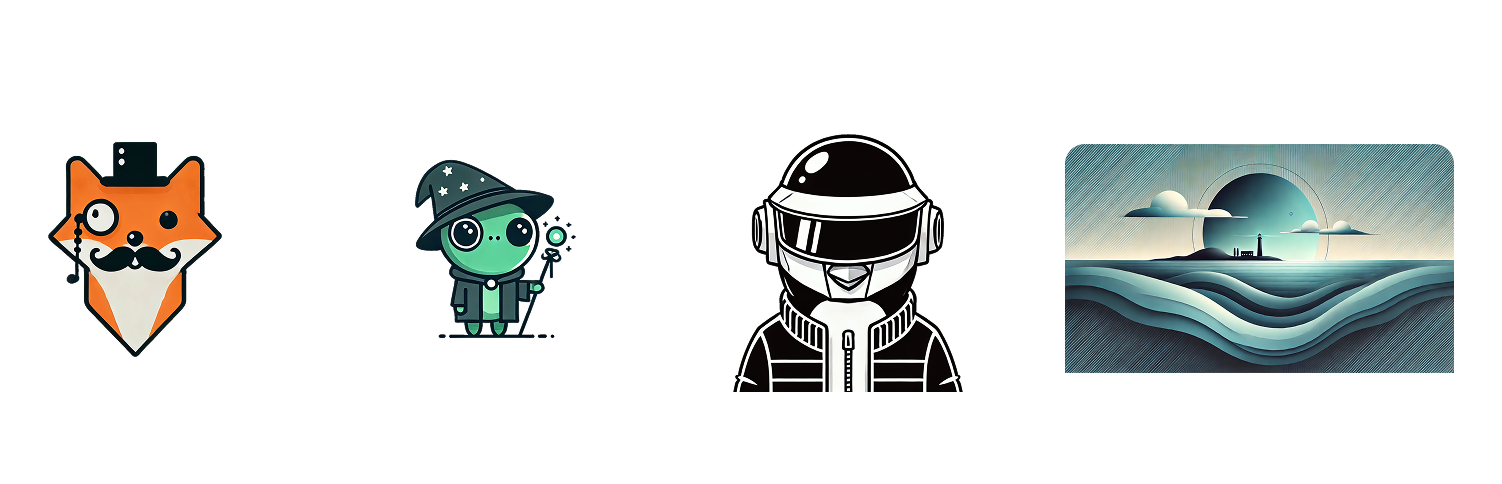
\includegraphics[width=0.8\linewidth]{Imagenes/Imagenes IA.png}
  \caption{Imágenes utilizadas}
  \label{fig:ER}
\end{figure}

\subsubsection{Módulo de logIn}

Este módulo permite el acceso de los usuarios que ya están registrados en el prototipo mediante correo electrónico y contraseña. La interfaz presenta un formulario simple, con campos identificados para el ingreso de credenciales. Además, se incluyen enlaces a las secciones “¿Olvidaste tu contraseña?” y “Regístrate”, que permiten respectivamente recuperar el acceso en caso de olvido y crear una nueva cuenta

\begin{figure}[H]
  \centering
  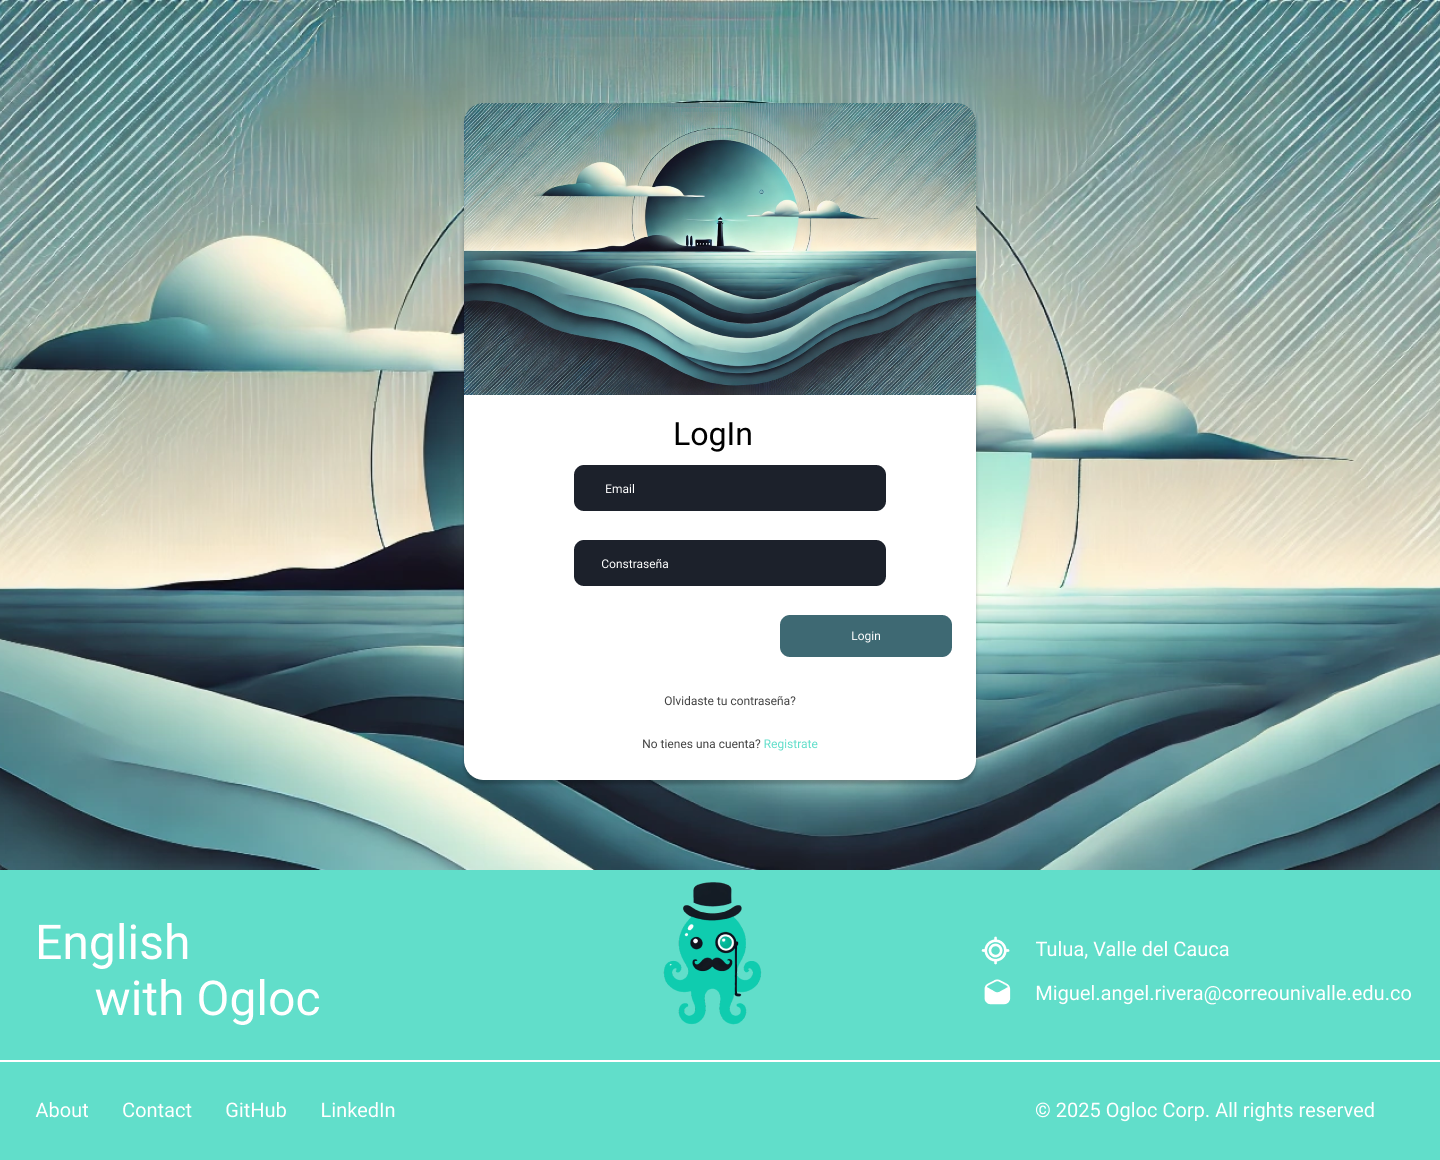
\includegraphics[width=0.8\linewidth]{Imagenes/Vista login.png}
  \caption{Mockup LogIn}
  \label{fig:ER}
\end{figure}

\subsubsection{Módulo de Registro}

El módulo de registro permite a los nuevos usuarios crear una cuenta en el prototipo mediante un formulario sencillo y accesible. Este formulario está compuesto por los campos: nombre completo, nombre de usuario (username), correo electrónico y contraseña. Cada uno de estos campos está diseñado para facilitar el ingreso de datos de manera clara y eficiente. Asimismo, se implementan validaciones básicas para asegurar que la información ingresada sea válida y coherente.

\begin{figure}[H]
  \centering
  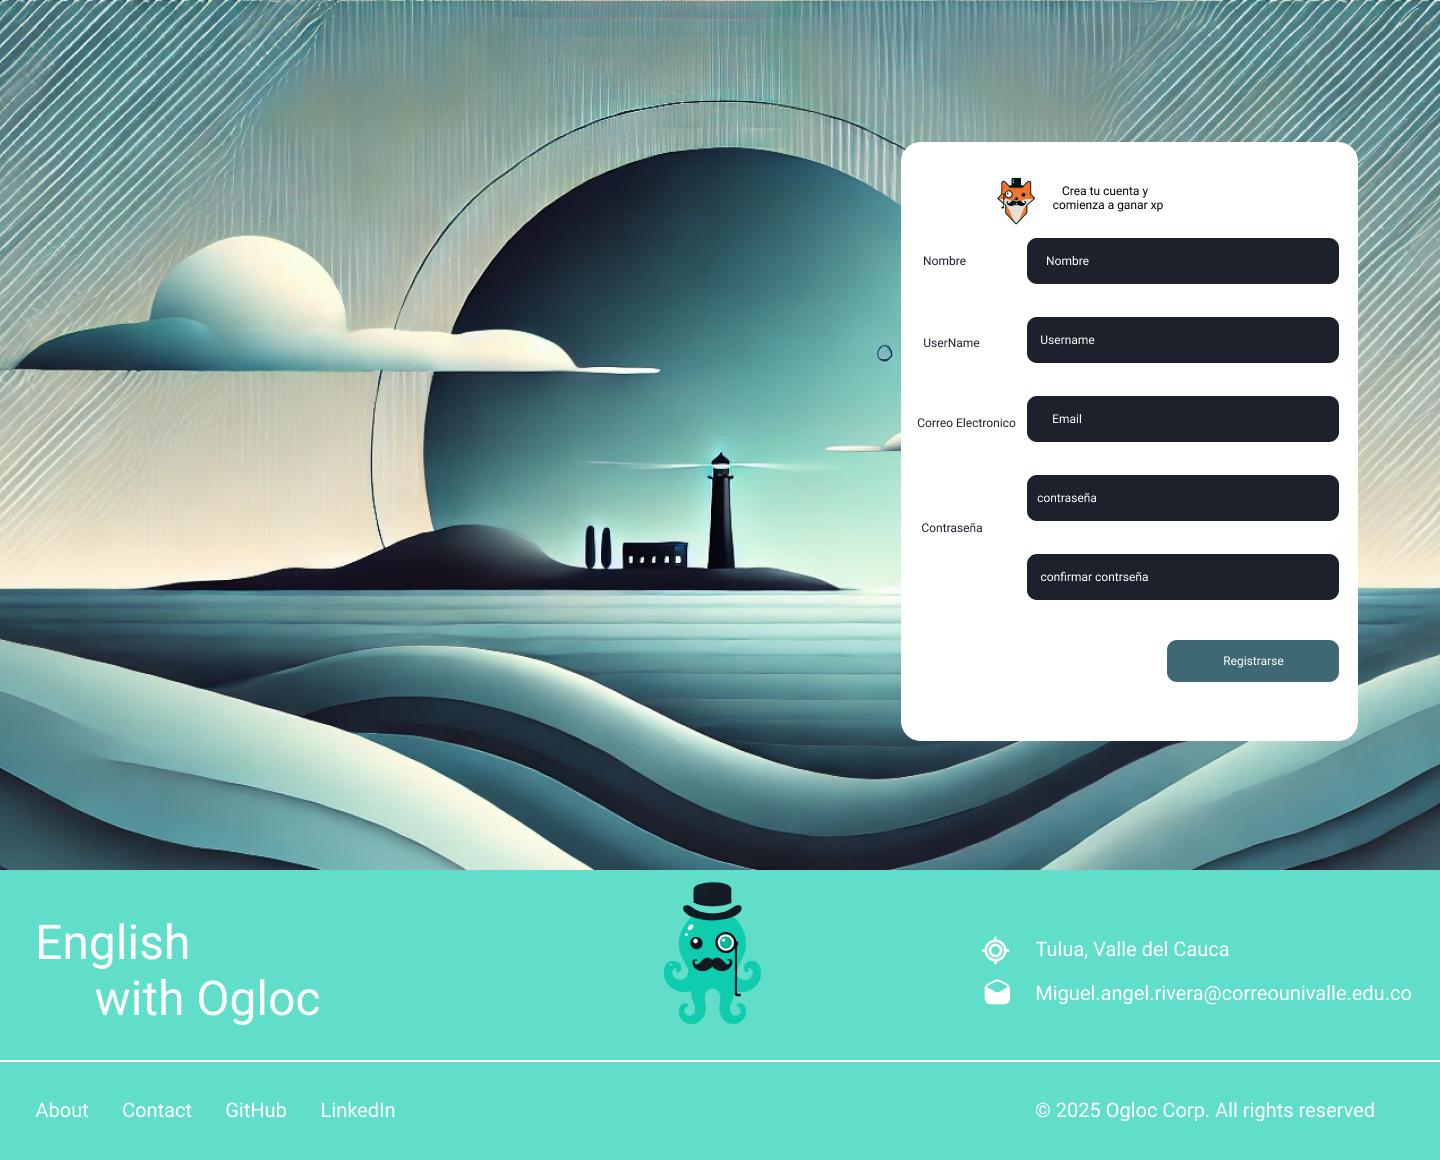
\includegraphics[width=0.6\linewidth]{Imagenes/Vista Registro.png}
  \caption{Mockup de Registro}
  \label{fig:ER}
\end{figure}


\subsubsection{Módulo perfil de usuario}

Este módulo permite al usuario visualizar y gestionar la información asociada a su cuenta. Desde esta sección, el usuario puede consultar datos como su nombre, nombre de usuario y su progreso dentro de la plataforma. Además, se incluye la posibilidad de editar algunos de estos datos o acceder a opciones adicionales como eliminar la cuenta.

\begin{figure}[H]
  \centering
  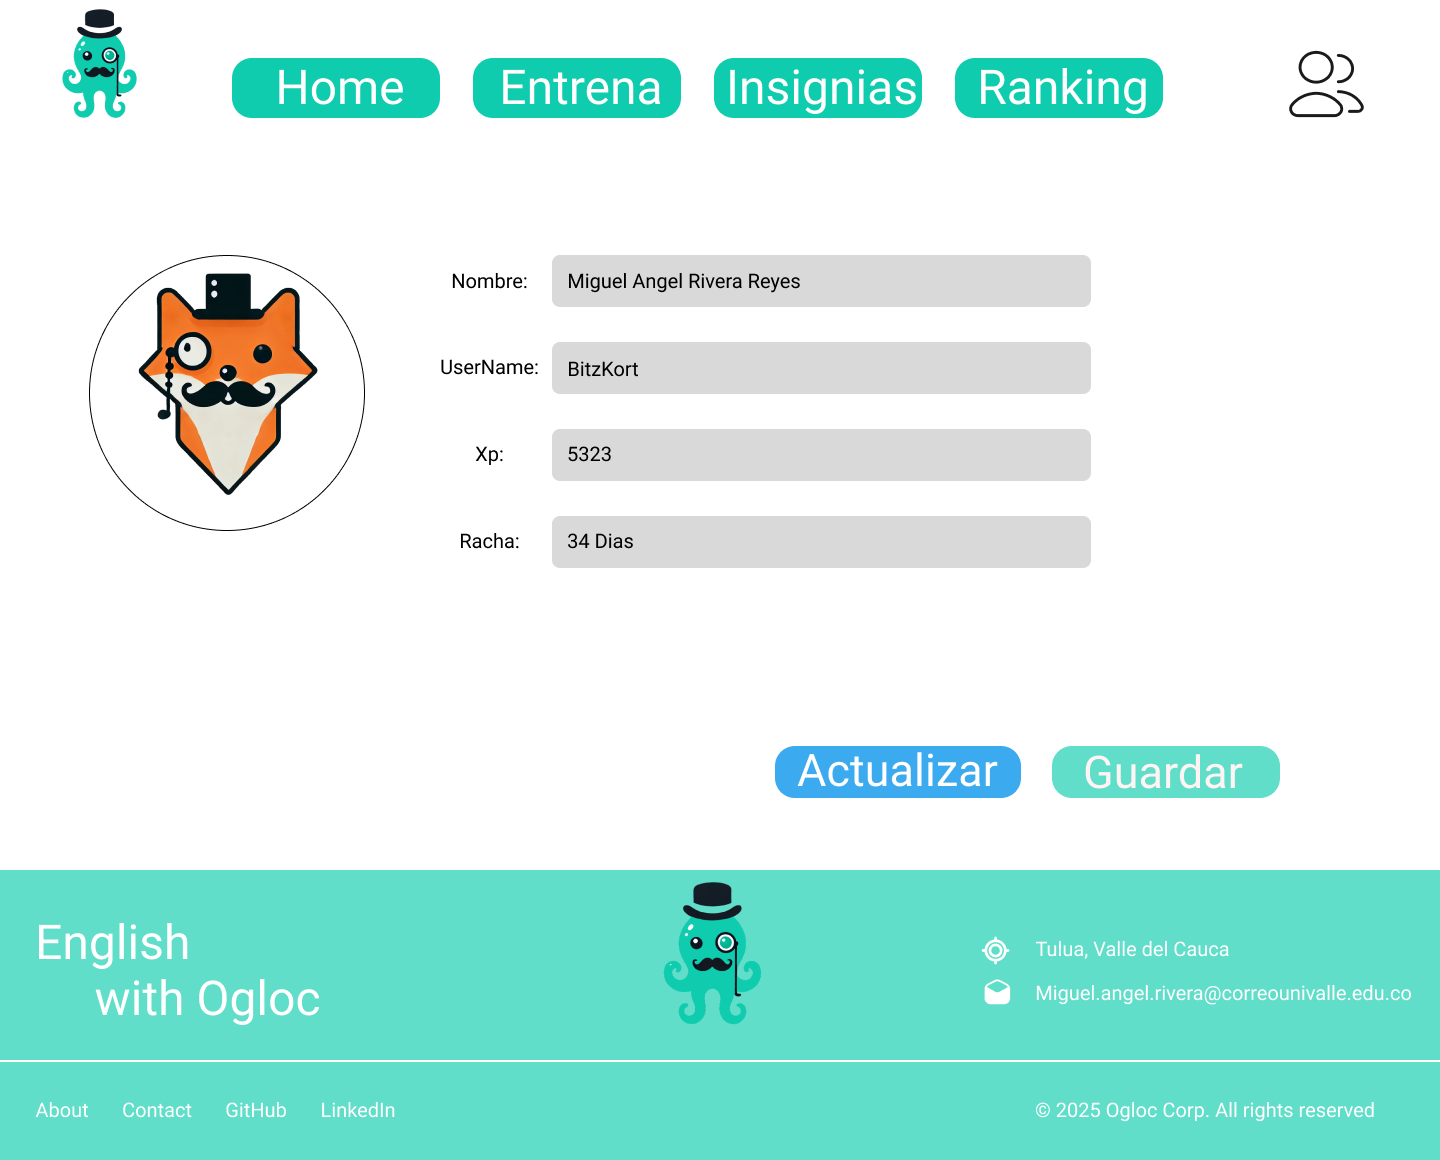
\includegraphics[width=0.5\linewidth]{Imagenes/vista perfil.png}
  \caption{Mockup perfil de usuario}
  \label{fig:ER}
\end{figure}

\subsubsection{Módulo preguntas}

Este módulo corresponde a la vista en la que se presentan las preguntas de cada lección , el usuario interactúa directamente con el contenido de aprendizaje respondiendo las preguntas que conforman una lección por medio del micrófono. Las preguntas se muestran una a una, de forma clara y ordenada.

\begin{figure}[H]
  \centering
  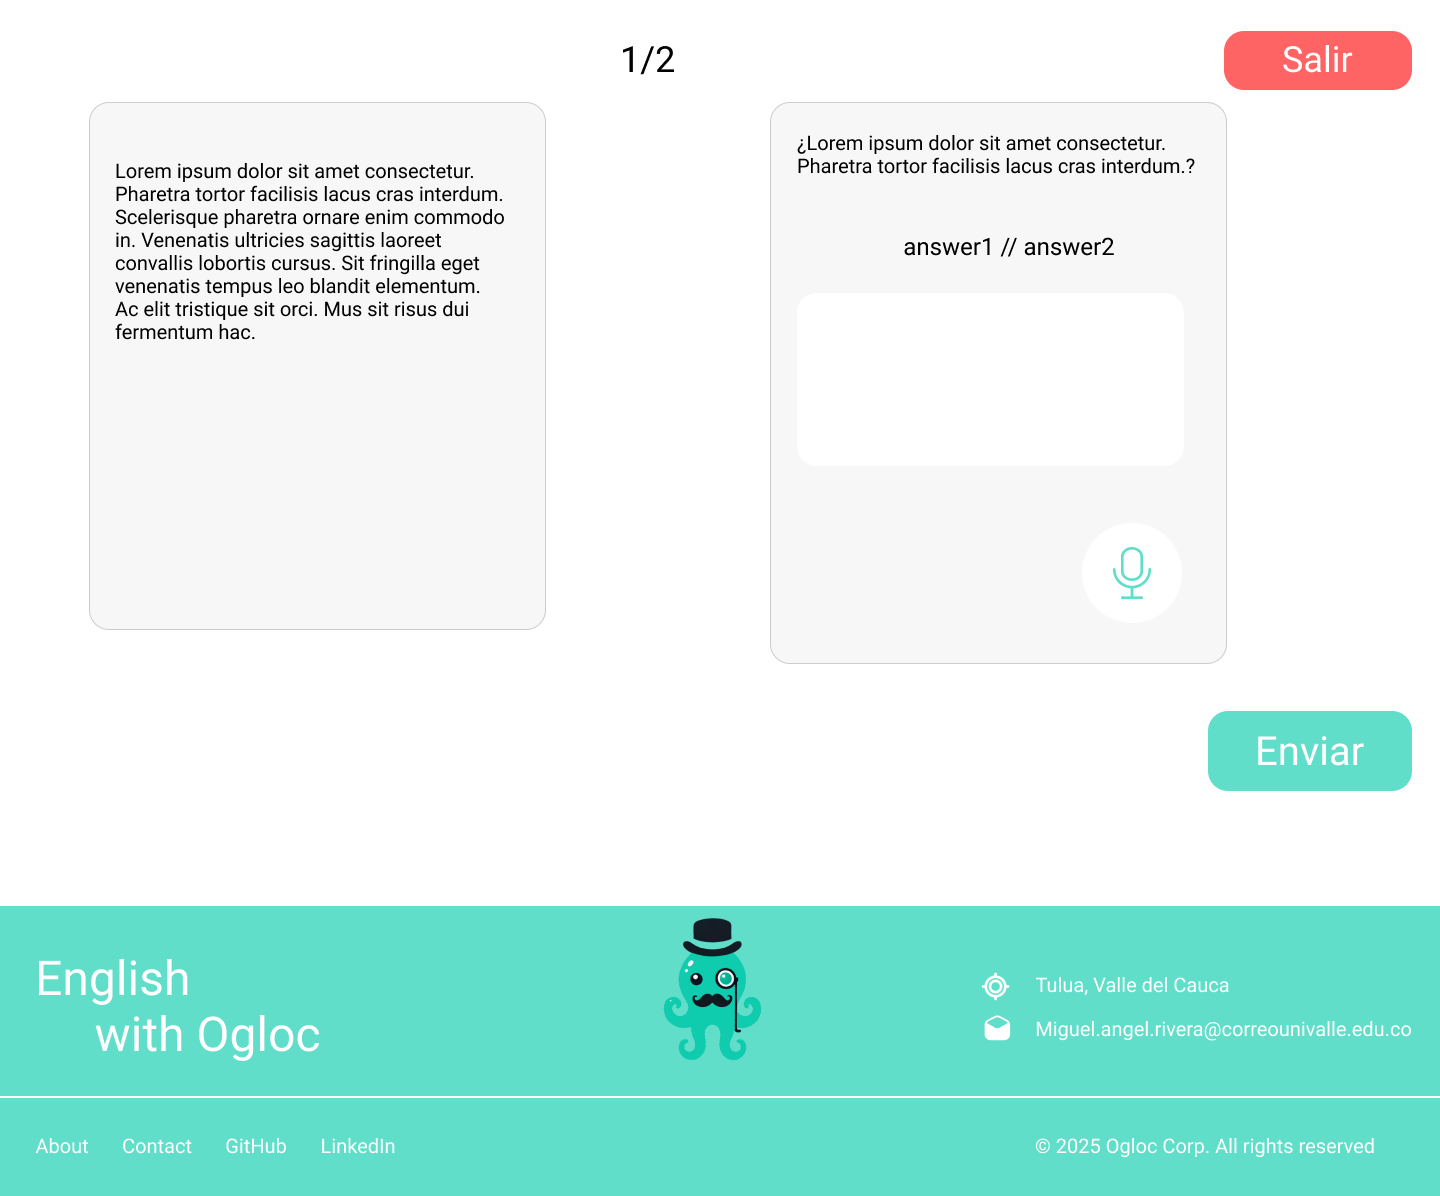
\includegraphics[width=0.6\linewidth]{Imagenes/Vista preguntas.png}
  \caption{Mockup vista preguntas}
  \label{fig:ER}
\end{figure}

\subsubsection{Módulo principal (home)}

Este módulo representa la página principal del prototipo, donde el usuario puede visualizar de forma general las funcionalidades más relevantes de la aplicación. En esta vista se presentan las lecciones disponibles para realizar, organizadas de manera que faciliten su acceso y comprensión. Además, se incluyen secciones dedicadas a las insignias obtenidas por el usuario, así como un acceso al pool de preguntas incorrectas, lo que permite reforzar los conocimientos previamente evaluados. Finalmente, se muestra un ranking global con los usuarios que han acumulado mayor experiencia (exp), promoviendo la motivación y el sentido de competencia entre los participantes.


\begin{figure}[H]
  \centering
  \includegraphics[width=0.5\linewidth]{Imagenes/Vista home.png}
  \caption{Mockup home}
  \label{fig:ER}
\end{figure}

\newpage
\subsubsection{Módulo Insignias}

Este módulo está dedicado a la visualización de las insignias que el usuario ha obtenido a lo largo de su progreso en la plataforma. Las insignias se otorgan en función de la cantidad de experiencia (exp) acumulada, la cual se incrementa a medida que el usuario responde correctamente las preguntas de las lecciones. Este sistema de recompensas tiene como objetivo incentivar la participación constante y reconocer el esfuerzo del usuario, proporcionando una representación visual de sus logros dentro de la aplicación. Las insignias se muestran de manera ordenada, permitiendo identificar tanto las obtenidas como las que aún están por desbloquear.

\begin{figure}[H]
  \centering
  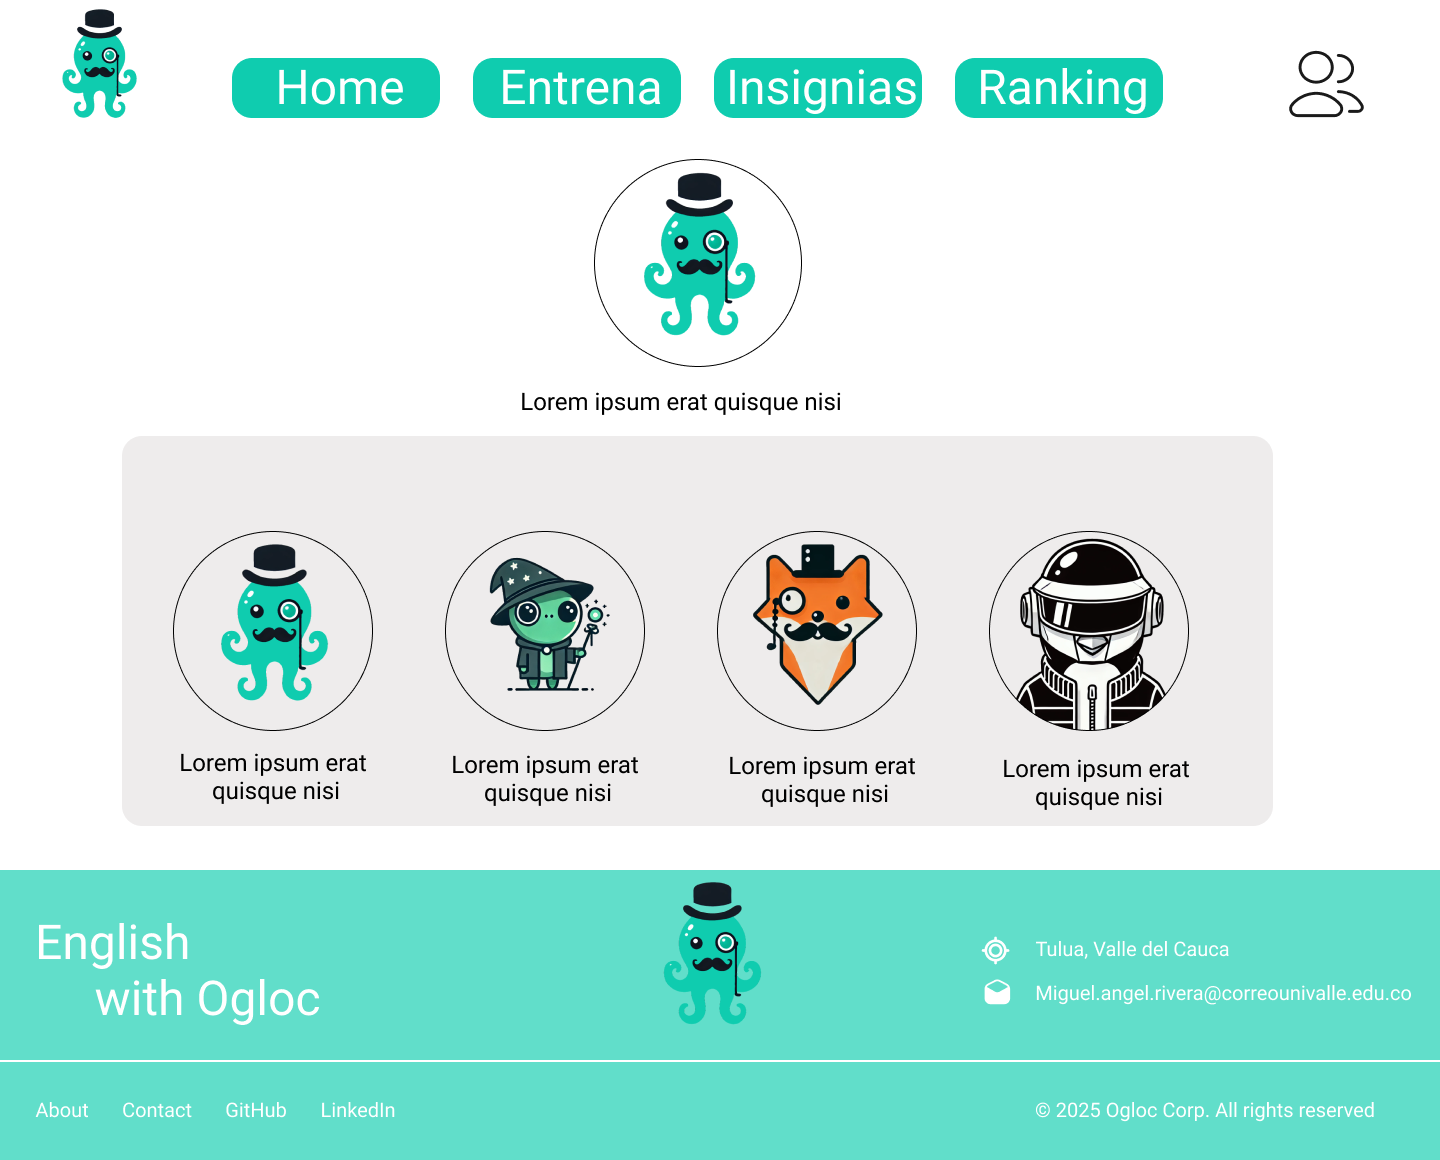
\includegraphics[width=0.6\linewidth]{Imagenes/Vista insignias.png}
  \caption{Mockup vista Insignias}
  \label{fig:ER}
\end{figure}